\section{Estimating Character-Dependent Speciation \& Extinction Rates}

\subsection{Outline}

This tutorial describes how to specify a character-dependent branching-process models in \RevBayes;
a birth-death process where diversification rates are dependent on the state of a discrete character \citep{Maddison2007,Fitzjohn2012,Beaulieu2016}.
The probabilistic graphical model is given for this tutorial.
Finally, you will estimate character-dependent speciation and extinction rates using Markov chain Monte Carlo (MCMC).


\subsection{Requirements}
We assume that you have read and hopefully completed the following tutorials:
\begin{itemize}
\item \href{https://github.com/revbayes/revbayes_tutorial/raw/master/tutorial_TeX/RB_Getting_Started/RB_Getting_Started.pdf}{Getting started}
\item \href{https://github.com/revbayes/revbayes_tutorial/raw/master/tutorial_TeX/RB_Basics_Tutorial/RB_Basics_Tutorial.pdf}{\Rev basics}
\item \href{https://github.com/revbayes/revbayes_tutorial/raw/master/tutorial_TeX/RB_DiversificationRate_Tutorial/RB_DiversificationRate_Tutorial.pdf}{Basic Diversification Rate Estimation}
\end{itemize}
Note that the \href{https://github.com/revbayes/revbayes_tutorial/raw/master/tutorial_TeX/RB_Basics_Tutorial/RB_Basics_Tutorial.pdf}{\Rev basics tutorial} introduces the basic syntax of \Rev but does not cover any phylogenetic models.
You may skip the \href{https://github.com/revbayes/revbayes_tutorial/raw/master/tutorial_TeX/RB_Basics_Tutorial/RB_Basics_Tutorial.pdf}{\Rev basics tutorial} if you have some familiarity with \R.
We tried to keep this tutorial very basic and introduce all the language concepts and theory on the way.
You may only need the \href{https://github.com/revbayes/revbayes_tutorial/raw/master/tutorial_TeX/RB_Basics_Tutorial/RB_Basics_Tutorial.pdf}{\Rev basics tutorial} for a more in-depth discussion of concepts in \Rev.


%%%%%%%%%%%%%%
%%   Data   %%
%%%%%%%%%%%%%%
\section{Data and files}

We provide the data file(s) which we will use in this tutorial.
You may want to use your own data instead.
In the \cl{data} folder, you will find the following files
\begin{itemize}
\item \href{https://github.com/revbayes/revbayes_tutorial/raw/master/RB_DiversificationRate_CharacterDependent_Tutorial/data/primates\_tree.nex}{primates\_tree.nex}: Dated primates phylogeny including 233 out of 367 species from \cite{MagnusonFord2012}.
\item \href{https://github.com/revbayes/revbayes_tutorial/raw/master/RB_DiversificationRate_CharacterDependent_Tutorial/data/primates_habitat.nex}{primates\_habitat.nex}: Habitat data from \cite{MagnusonFord2012}. There is also a larger set of \href{https://github.com/revbayes/revbayes_tutorial/raw/master/RB_DiversificationRate_CharacterDependent_Tutorial/data/primates_morph.nex}{discrete morphological characters}. The type of characters are described in the file \href{https://github.com/revbayes/revbayes_tutorial/raw/master/RB_DiversificationRate_CharacterDependent_Tutorial/data/primates_morph_description.txt}{primates\_morph\_description.txt}.
\end{itemize}


\impmark{Open the tree \cl{data/primates\_tree.nex} in FigTree.}

\impmark{Open the character data file \cl{data/primates\_morph.nex} in a text editor.}


\bigskip
\section{The Theory behind Character-dependent diversification rate models}\label{sec:BiSSE_Theory}

\RevBayes implements the multi-state extension of \BiSSE, just as implemented in \diversitree. 
The main differences are just which priors you use on the parameters and the inference procedure, \IE the specifics of the MCMC algorithm.
Here we will first describe the general theory about the model, borrowing heavily from the supplementary material of \cite{Moore2016}.
You may want to skip over this section if you are not interested in math behind.
Then we will show how to run this analysis in \RevBayes.
\begin{figure}[h!]
\centering
\fbox{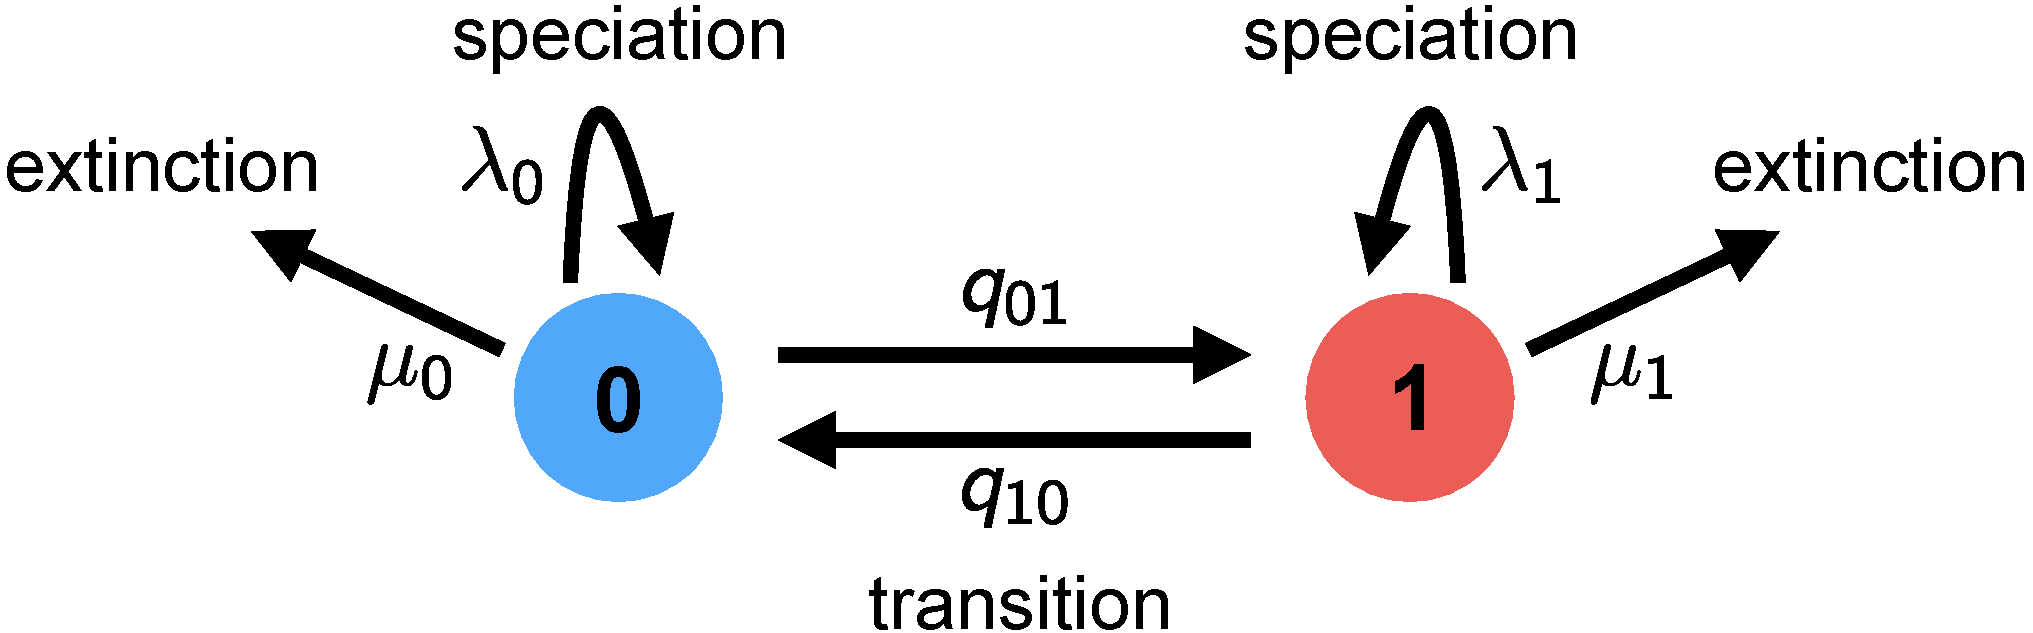
\includegraphics[width=\textwidth]{\ResourcePath figures/BiSSE.pdf}}
\caption{\small A schematic overview of the \BiSSE model. Each lineage has a binary state associated to it and thus can either be in state 0 (blue) or state 1 (red). When a lineage is in state 0 (blue), it can either (a) speciate with rate $\lambda_0$ which results into two descendant lineage both being in state 0 (blue); (b) it can go extinct with rate $\mu_0$; or (c) it can switch the state to 1 (red) with rate $q_{01}$. The same type of events are possible when a lineage is in state 1 (red) but with rate $\lambda_1$, $\mu_1$, and $q_{10}$ respectively.}
\label{fig:BiSSE_Schematic}
\end{figure}

%%%%%%%%%%%%%%%%%%%%%%%%%%%%
%%%    LIKELIHOOD  FN    %%%
%%%%%%%%%%%%%%%%%%%%%%%%%%%%
\subsection{Likelihood function}\label{section:likelihood}
We introduce the theory and likelihood function of the \BiSSE (Binary State Speciation and Extinction) model developed in \cite{Maddison2007}.
The \BiSSE model assumes a finite number of states (two; one for each of the binary states), where the states of each extant species is known (indeed, it is an observed discrete trait).
The general approach adopted by \BiSSE models is to derive a set of ordinary differential equations (ODEs) that describe how the probability of observing a descendant clade changes along a branch in the observed phylogeny.
Each equation in this set describes how the probability of observing the clade changes through time if it is in a particular state over that time period; collectively, these equations are called $\frac{ \mathrm{d}D_{N,i}(t)}{\mathrm{d}t}$, where the subscript $N$ refers to the descendant clade and the subscript $i$ refers to $i^\text{th}$ state.

Computing the likelihood proceeds by establishing an initial value problem: in principle, if we know the probabilities of observing a lineage at some specific time (\EG the present), and know how those probabilities change over time (described by the ODEs), then we can compute the probabilities of observing those lineages at some earlier time (\EG the root).
Assuming that there are exactly $k$ possible states, we initialize $k$ probabilities at each tip in the phylogeny; we then compute how each of those $k$ probabilities changes down each branch in the tree using the above set of $k$ ODEs.
At each node in the tree, we take the product of each of the $k$ probabilities for the descendants of that node (multiplied by the instantaneous speciation rate for each of the $k$ states to account for the observed speciation event at the node) as the initial values for the ancestral branch subtending that node.
Proceeding in this way down the tree results in a set of $k$ probabilities at the root; these $k$ probabilities represent the probability of observing the phylogeny conditional on the root being in each of the states (\IE the $i^\text{th}$ conditional probability is the probability of observing the tree given that the root is in state $i$).
The overall likelihood of the tree is a weighted average of the $k$ probabilities at the root, where the weighting scheme represents the assumed probability that the root was in each of the $k$ states.

As with all birth-death process models, special care must be taken to account for the possibility of extinction.
Specifically, the above ODEs must accommodate lineages that may arise along each branch in the tree that subsequently go extinct before the present (and so are unobserved).
This requires a second set of $k$ ODEs, $\frac{ \mathrm{d}E_{i}(t)}{\mathrm{d}t}$, which define how the probability of extinction in process $i$ changes over time.
These ODEs must be solved to compute the differential equations $\frac{ \mathrm{d}D_{N,i}(t)}{\mathrm{d}t}$, as we will demonstrate when we derive both sets of equations in the following sections.

This framework therefore requires four distinct pieces of information to compute the likelihood of the data:
%	\begin{enumerate}
%		\item A set of ordinary differential equations describing how the probability of the data (observed lineages) changes through time, $\frac{ \mathrm{d}D_{N,i}(t)}{\mathrm{d}t}$.
%		\item A set of ordinary differential equations describing how the extinction probability of unobserved (extinct or unsampled) lineages changes through time, $\frac{ \mathrm{d}E_{i}(t)}{\mathrm{d}t}$.
%		\item An appropriate set of initial conditions.
%		\item An appropriate weighting scheme for the root probabilities.
%	\end{enumerate}

In the following sections we detail how each of these components is determined for increasingly complex birth-death process models.


\subsubsection{Binary-state space of diversification processes}
Consider a (time-independent) birth-death process with two possible states (\EG a binary state), with diversification rates $\{\lambda_0, \mu_0\}$ and $\{\lambda_1, \mu_1\}$.
We define $D_{N,0}(t)$ as the probability of observing lineage $N$ descending from a particular branch at time $t$, given that the lineage at that point is in state 0 (with rate parameters $\lambda_{0}$, and $\mu_{0}$).
To compute the probability of observing the lineage at some earlier point, $ D_{N,0}(t + \Delta t)$, we enumerate all possible events that could occur within the interval $\Delta t$.
Assuming that $\Delta t$ is small---so that the probability of any two events occurring in the interval is negligible---there are four possible scenarios within the interval:
\begin{enumerate}
	\item nothing happens in the interval;
	\item the process changes $0 \rightarrow 1$;
	\item a speciation event occurs and the left descendant subsequently goes extinct before the present, or;
	\item a speciation event occurs and the right descendant subsequently goes extinct before the present.
\end{enumerate}
We can thus compute $D_{N,0}(t + \Delta t)$ as (see \cite{Maddison2007} and \cite{FitzJohn2009} for a more complete elucidation):
\begin{align}
	D_{N,0}(t + \Delta t) = & \;(1 - \mu_0\Delta t) \times & \text{in all cases, no extinction of the observed lineage} \label{equation:ProbDeltaT} \\
			    		   & \;[  (1 - q\Delta t)(1 - \lambda_0\Delta t)D_{N,0}(t) & \text{Case (1) nothing happens} \nonumber\\
						   & \; + q_{01}\Delta t (1 - \lambda_0\Delta t)D_{N,1}(t) & \text{Case (2) process change but no speciation} \nonumber\\
						   & \; + (1 - q_{01}\Delta t)\lambda_0\Delta t E_0(t)D_{N,0}(t) & \text{Case (3) no process change, speciation, extinction} \nonumber\\
						   & \; + (1 - q\Delta t)\lambda_0\Delta t E_0(t)D_{N,0}(t)] & \text{Case (4) no process change, speciation, extinction} \nonumber
\end{align}
A matching equation can be written down for $D_{N,1}(t+\Delta t)$.

Define $E_0(t)$ as the probability that a lineage in state 0 at time $t$ goes extinct before the present.
To determine the extinction probability at an earlier point, $E_0(t+\Delta t)$, we can again enumerate all the possible events in the interval $\Delta t$:
\begin{enumerate}
	\item the lineage goes extinct within the interval;
	\item the lineage neither goes extinct nor speciates, resulting in a single lineage that must eventually go extinct before the present;
	\item the lineage neither goes extinct nor speciates, but there is a state change, resulting in a single lineage that must go extinct before the present, or;
	\item the lineage speciates in the interval, resulting in \emph{two} lineages that must eventually go extinct before the present.
\end{enumerate}

\begin{align}
	E_0(t + \Delta t) = &\; \mu_0\Delta t +	& \text{Case (1) extinction in the interval} \label{equation:ExtDeltaT}\\
				     & (1 - \mu_0\Delta t) \times & \text{no extinction in the interval and \dots} \nonumber\\
				     & \;[(1-q_{01}\Delta t)(1-\lambda_0\Delta t)E_0(t) & \text{Case (2) nothing happens, but subsequent extinction} \nonumber\\
				     & \;+ q_{01}\Delta t (1-\lambda_0\Delta t)E_1(t) & \text{Case (3) process change and subsequent extinction} \nonumber\\
				     & \;+ (1 - q\Delta t) \lambda_0\Delta t E_0(t)^2] & \text{Case (4) speciation and subsequent extinctions} \nonumber
\end{align}
Again, a matching equation $E_1(t+\Delta t)$ can be written down.

\subsection{Extension to a multi-state birth-death process}
We can expand the \BiSSE model to accommodate an arbitrary number of processes, $k$, by writing a set of $k$ difference equations $D_{N,0}(t+\Delta t), D_{N,1}(t+\Delta t), \ldots, D_{N,k}(t+\Delta t)$.
%\begin{align}
%		D_{N,i}(t + \Delta t) = & \;(1 - \mu_i\Delta t) \times \label{equation:DKStates} \\
%		& \;[  (1 - \sum\limits_{j \neq i}^k q_{ij}\Delta t)(1 - \lambda_i\Delta t)D_{N,i}(t) \nonumber\\
%		& \; + (1 - \lambda_i\Delta t)  \sum\limits_{j \neq i}^k q_{ij}\Delta t D_{N,j}(t) \nonumber\\
%		& \; + 2 (1 - \sum\limits_{j \neq i}^k q\Delta t) \lambda_i\Delta t E_i(t)D_{N,i}(t)] \nonumber
%\end{align}
%along with $E_0(t+\Delta t), E_1(t+\Delta t), \ldots, E_k(t+\Delta t)$:
%\begin{align}
%	E_i(t + \Delta t) = &\; \mu_i\Delta t +	\label{equation:ExtKStates}	\\
%				    	    & (1 - \mu_i\Delta t) \times \nonumber\\
%					    & \;[(1-\sum\limits_{j \neq i}^k q_{ij}\Delta t)(1-\lambda_i\Delta t)E_i(t) \nonumber\\
%					    & \;+ (1-\lambda_i\Delta t) \sum\limits_{j \neq i}^k q_{ij}\Delta t E_j(t) \nonumber\\
%					    & \;+ (1 - \sum\limits_{j \neq i}^k q\Delta t) \lambda_i\Delta t E_i(t)^2] \nonumber
%\end{align}
The resulting differential equations are (see \cite{Maddison2007} for the two-process case and \cite{FitzJohn2010} for the $k$-process case):
\begin{align*}
	\frac{\mathrm{d}D_{N,i}(t)}{\mathrm{d}t} = & - \left(\lambda_i + \mu_i + \sum\limits_{j \neq i}^k q\right)D_{N,i}(t) + 2\lambda_iE_i(t)D_{N,i}(t) + \sum\limits_{i \neq j}^k q D_{N,j}(t) \\
   	\frac{\mathrm{d}E_i(t)}{\mathrm{d}t} = & - \left(\lambda_i + \mu_i + \sum\limits_{j \neq i}^k q \right)E_i(t) + \lambda_iE_i(t)^2 + \mu_i + \sum\limits_{i \neq j}^k q E_j(t)
\end{align*}

Initial probabilities are assigned according to the observed discrete states: if species $i$ has state $j$, then $D_{i,j}(0) = 1$ for the observed state (or $D_{i,j}(0) = \rho_j$ when species sampling is incomplete), and $D_{i,j}(0) = 0$ for all other ($\neq j$) states.
%If the state is not observable, then $D_{i,j}(0) = 1$ for all $j$, since all states have probability 1 of producing the observation; this is analogous to the treatment of missing or ambiguous states in conventional phylogenetic likelihood calculation, \emph{c.f.}, \cite{Felsenstein2004}.
Initial extinction probabilities are set to 0 (since there is no time for extinction to occur at the present) or to $1-\rho_i$ if incomplete taxon sampling is used. 
Root probabilities are either weighted using equal probabilities (uniformly), by a vector of pre-defined root stationary probabilities (informative), or by the stationary distribution of the model, to compute the overall likelihood of the data.


\begin{table}[t!]
	\centering
	\caption{\bf{\BiSSE model parameters and their interpretation}} \label{tab:param}
	\begin{tabular}{ l l l }
		\toprule
		Parameter & Interpretation \\
		\midrule
		$\Psi$ & Phylogenetic tree with divergence times.\\
		\rowcolor{gray!15} $T$ & The root age.\\
%		\rowcolor{gray!15} $\gamma$ & Prior mean of the Poisson rate $\Lambda$.\\
%		$\Lambda$ & Prior mean of the Poisson-distributed number $k$ of shift events.\\
		$q_{01}$ & The rate of shifts from 0 to 1.\\
		\rowcolor{gray!15} $q_{10}$ & The rate of shifts from 1 to 0.\\
		$\lambda_0$ & Speciation rate for state 0.\\
		\rowcolor{gray!15} $\mu_0$ & Extinction rate for state 0.\\
		$\lambda_1$ & Speciation rate for state 1.\\
		\rowcolor{gray!15} $\mu_1$ & Extinction rate for state 1.\\
	\end{tabular}
\end{table}


\section{Character-dependent diversification rates}\label{sec:CDBDP}
Now let's start to analyze an example in \RevBayes using the BiSSE model.

\subsection{Read the tree}

Begin by reading in the observed tree and the morphological data. 
We have both stored in separate nexus files.
{\tt \begin{snugshade*}
\begin{lstlisting}
observed_phylogeny <- readTrees("data/primates_tree.nex")[1]
data <- readCharacterData("data/primates_solitariness.nex")
\end{lstlisting}
\end{snugshade*}}
Note, the character-dependent birth-death process currently uses always the first character/site in the alignment file.
We have therefore split the morphological dataset into several small files that include only one morphological character each.

From the tree, we can get some helpful variables:
{\tt \begin{snugshade*}
\begin{lstlisting}
taxa <- observed_phylogeny.taxa()
\end{lstlisting}
\end{snugshade*}}

Additionally, we can initialize an iterator variable for our vector of moves and monitors:
{\tt \begin{snugshade*}
\begin{lstlisting}
mvi = 0
mni = 0
\end{lstlisting}
\end{snugshade*}}

Finally, we create a helper variable that specifies the number of states that the morphological character has.
{\tt \begin{snugshade*}
\begin{lstlisting}
NUM_STATES = 2
\end{lstlisting}
\end{snugshade*}}
Using this variable we can easily change our script to use a different morphological character with a different number of states.
We will also use this variable in our second example on hidden-state speciation and extinction model. 



\subsection{Specifying the model}

The basic idea behind the model in this example is that speciation and extinction rates are dependent on a binary character \citep{Maddison2007}.


\subsubsection{Priors on rates}
We start by specifying prior distributions on the diversification rates.
We will assume here an identical prior distribution on the speciation and extinction rate.
Furthermore, we will use a normal distribution as the prior distribution on the log of the speciation and extinction rate.
Hence, we will use a mean of $\frac{\ln(\frac{\text{\#Taxa}}{2})}{\text{tree-age}}$ which is the expected net-diversification rate.
{\tt \begin{snugshade*}
\begin{lstlisting}
rate_mean <- ln( ln(367.0/2.0) / observed_phylogeny.rootAge() )
rate_sd <- 2.0
\end{lstlisting}
\end{snugshade*}}
Now we can specify our character-specific specification and extinction rate parameters.
As we just said before, we are going to use normal distributions for the prior on the log-speciation and log-extinction rate.
Here we will use a \cl{for}-loop to specify speciation and extinction parameters for each character, \EG two in a binary state case.
{\tt \begin{snugshade*}
\begin{lstlisting}
for (i in 1:NUM_STATES) {
    
     ### Create a lognormal distributed variable for the diversification rate
    log_speciation[i] ~ dnNormal(mean=rate_mean,sd=rate_sd) 
    speciation[i] := exp( log_speciation[i] )
    moves[++mvi] = mvSlide(log_speciation[i],delta=0.20,tune=true,weight=3.0)

    ### Create a lognormal distributed variable for the turnover rate
    log_extinction[i] ~ dnNormal(mean=rate_mean,sd=rate_sd) 
    extinction[i] := exp( log_extinction[i] )
    moves[++mvi] = mvSlide(log_extinction[i],delta=0.20,tune=true,weight=3.0)

}
\end{lstlisting}
\end{snugshade*}}
Great! Now we have create our main variables of interest, the state-specific speciation and extinction rate variables with some meaningful prior distributions. 
Additionally, we have already created moves on these variables.
So we can now turn our focus on the remaining variables of the model.

Next, we specify the transition rates $q_{01}$ and $q_{10}$ between the two states 0 and 1.
Each transition rate between observed states is drawn rom an exponential distribution with a mean of 10 character state transitions over the entire tree. 
We hope that this is a reasonable prior but also leaves enough uncertainty in our prior knowledge.
(You may want to compare the posterior to the prior and/or check the resulting posterior estimates for different choices of the prior!)
{\tt \begin{snugshade*}
\begin{lstlisting}
rate_pr := observed_phylogeny.treeLength() / 10
rate_12 ~ dnExponential(rate_pr)
rate_21 ~ dnExponential(rate_pr)
\end{lstlisting}
\end{snugshade*}}
For both rate variable we specify a scaling move.
{\tt \begin{snugshade*}
\begin{lstlisting}
moves[++mvi] = mvScale( rate_12, weight=2 )
moves[++mvi] = mvScale( rate_21, weight=2 )
\end{lstlisting}
\end{snugshade*}}
Finally, we build a rate matrix for the relative-rate of change between categories.
This is because we need a rate matrix in our state-dependent birth-death process.
{\tt \begin{snugshade*}
\begin{lstlisting}
rate_matrix := fnFreeBinary( [rate_12, rate_21 ], rescaled=false)
\end{lstlisting}
\end{snugshade*}}
A specific note here is that we do not rescale the rate matrix. 
This is very important because otherwise rate matrices, as used for molecular evolution, are always rescaled to have an average rate of 1.0.
If such a rescaled rate matrix was used, then you need to provide an overall rate scalar $\delta$.

\subsubsection{Prior on the root state}
Create a variable with the prior probabilities of each rate category at the root.
We are using a flat Dirichlet distribution as the prior on each state.
In this case we are actually estimating the prior frequencies of the root states.
There has been some discussion about this in \cite{FitzJohn2009}.
You could also fix the prior probabilities for the root states to be equal (generally not recommended), or use empirical state frequencies. 
{\tt \begin{snugshade*}
\begin{lstlisting}
rate_category_prior ~ dnDirichlet( rep(1,NUM_STATES) )
moves[++mvi] = mvDirichletSimplex(rate_category_prior,tune=true,weight=2)
\end{lstlisting}
\end{snugshade*}}

\subsubsection{Incomplete Taxon Sampling}

We know that we have sampled 233 out of 367 living primate species. 
To account for this we can set the sampling parameter as a constant node with a value of 233/367
{\tt \begin{snugshade*}
\begin{lstlisting}
rho <- observed_phylogeny.ntips()/367
\end{lstlisting}
\end{snugshade*}}


\subsubsection{Root age}

The birth-death process requires a parameter for the root age.
In this exercise we use a fix tree and thus we know the age of the tree.
Hence, we can get the value for the root from the \citet{MagnusonFord2012} tree.
{\tt \begin{snugshade*}
\begin{lstlisting}
root <- observed_phylogeny.rootAge()
\end{lstlisting}
\end{snugshade*}}

\subsubsection{The time tree}

Now we have all of the parameters we need to specify the full episodic birth-death model. 
We initialize the stochastic node representing the time tree.
{\tt \begin{snugshade*}
\begin{lstlisting}
timetree ~ dnCDBDP( rootAge           = root,
                    speciationRates   = speciation,
                    extinctionRates   = extinction, 
                    Q                 = rate_matrix,
                    pi                = rate_category_prior,
                    delta             = 1.0,
                    rho               = rho,
                    condition         = "survival",
                    taxa              = taxa )
\end{lstlisting}
\end{snugshade*}}
And then we attach data to it.
{\tt \begin{snugshade*}
\begin{lstlisting}
timetree.clamp( observed_phylogeny )
timetree.clampCharData( data )
\end{lstlisting}
\end{snugshade*}}

Finally, we create a workspace object of our whole model using the \cl{model()} function. 
{\tt \begin{snugshade*}
\begin{lstlisting}
mymodel = model(rate_matrix)
\end{lstlisting}
\end{snugshade*}}

The \cl{model()} function traversed all of the connections and found all of the nodes we specified. 


\subsection{Running an MCMC analysis}

\subsubsection{Specifying Monitors}

For our MCMC analysis, we set up a vector of \emph{monitors} to record the states of our Markov chain. 
The first monitor will model all numerical variables, specifically we are interested in speciation rates $\lambda_0$ and $\lambda_1$ as well as the extinction rates $\mu_0$ and $\mu_1$.
{\tt \begin{snugshade*}
\begin{lstlisting}
monitors[++mni] = mnModel(filename="output/primates_BiSSE.log", printgen=1)
\end{lstlisting}
\end{snugshade*}}
The second monitor is a new type of monitor: an joint-ancestral-states monitor.
This monitor takes a draw from joint posterior distribution of the ancestral states.
Thus, with this output file we will be able to make a nice plot with ancestral states.
{\tt \begin{snugshade*}
\begin{lstlisting}
monitors[++mni] = mnJointConditionalAncestralState(tree=timetree, cdbdp=timetree, type="Standard", printgen=1, withTips=true, withStartStates=false, filename="output/anc_states_primates_BiSSE.log")
\end{lstlisting}
\end{snugshade*}}
Finally, we add a screen monitor showing some updates during the MCMC run.
{\tt \begin{snugshade*}
\begin{lstlisting}
monitors[++mni] = mnScreen(printgen=10, rate_12, rate_21, speciation, extinction)
\end{lstlisting}
\end{snugshade*}}

\subsubsection{Initializing and Running the MCMC Simulation}

With a fully specified model, a set of monitors, and a set of moves, we can now set up the MCMC algorithm that will sample parameter values in proportion to their posterior probability. 
The \cl{mcmc()} function will create our MCMC object:
{\tt \begin{snugshade*}
\begin{lstlisting}
mymcmc = mcmc(mymodel, monitors, moves)
\end{lstlisting}
\end{snugshade*}}

First, we will run a pre-burnin to tune the moves and to obtain starting values from the posterior distribution.
{\tt \begin{snugshade*}
\begin{lstlisting}
mymcmc.burnin(generations=5000,tuningInterval=200)
\end{lstlisting}
\end{snugshade*}}

Now, run the MCMC:
{\tt \begin{snugshade*}
\begin{lstlisting}
mymcmc.run(generations=20000)
\end{lstlisting}
\end{snugshade*}}


\subsubsection{Summarizing ancestral states}
After our MCMC run has finished, we read-in again our samples from the joint-ancestral-state posterior distribution.
{\tt \begin{snugshade*}
\begin{lstlisting}
anc_states = readAncestralStateTrace("output/anc_states_primates_BiSSE.log")
\end{lstlisting}
\end{snugshade*}}
Then we can use this trace and our fixed tree to compute the posterior probabilities of the ancestral states and prepare the output for plotting.
We will use the function called \cl{ancestralStateTree} which stores the tree with ancestral states automatically in a file.
{\tt \begin{snugshade*}
\begin{lstlisting}
anc_tree = ancestralStateTree(tree=observed_phylogeny, ancestral_state_trace_vector=anc_states, include_start_states=false, file="output/anc_states_primates_BiSSE_results.tree", burnin=0, summary_statistic="MAP", site=0)
\end{lstlisting}
\end{snugshade*}}


\subsubsection{Plotting ancestral states}

Let us first plot the ancestral states mapped on the phylogeny.
We will use \R and the package \RevGadgets.
Execute the following code in \R.
\definecolor{shadecolor}{RGB}{200,200,200}
{\tt \begin{snugshade*}
\begin{lstlisting}
library(RevGadgets)

tree_file = "output/anc_states_primates_BiSSE_results.tree"

plot_ancestral_states(tree_file, summary_statistic="MAP",
                      tip_label_size=0,
                      xlim_visible=NULL,
                      node_label_size=0,
                      show_posterior_legend=TRUE,
                      node_size_range=c(2, 6),
                      alpha=0.75)

output_file = "RevBayes_Anc_States_BiSSE.pdf"
ggsave(output_file, width = 11, height = 9)
\end{lstlisting}
\end{snugshade*}}
\definecolor{shadecolor}{RGB}{183,207,237}
\begin{figure}[h!]
\centering
\fbox{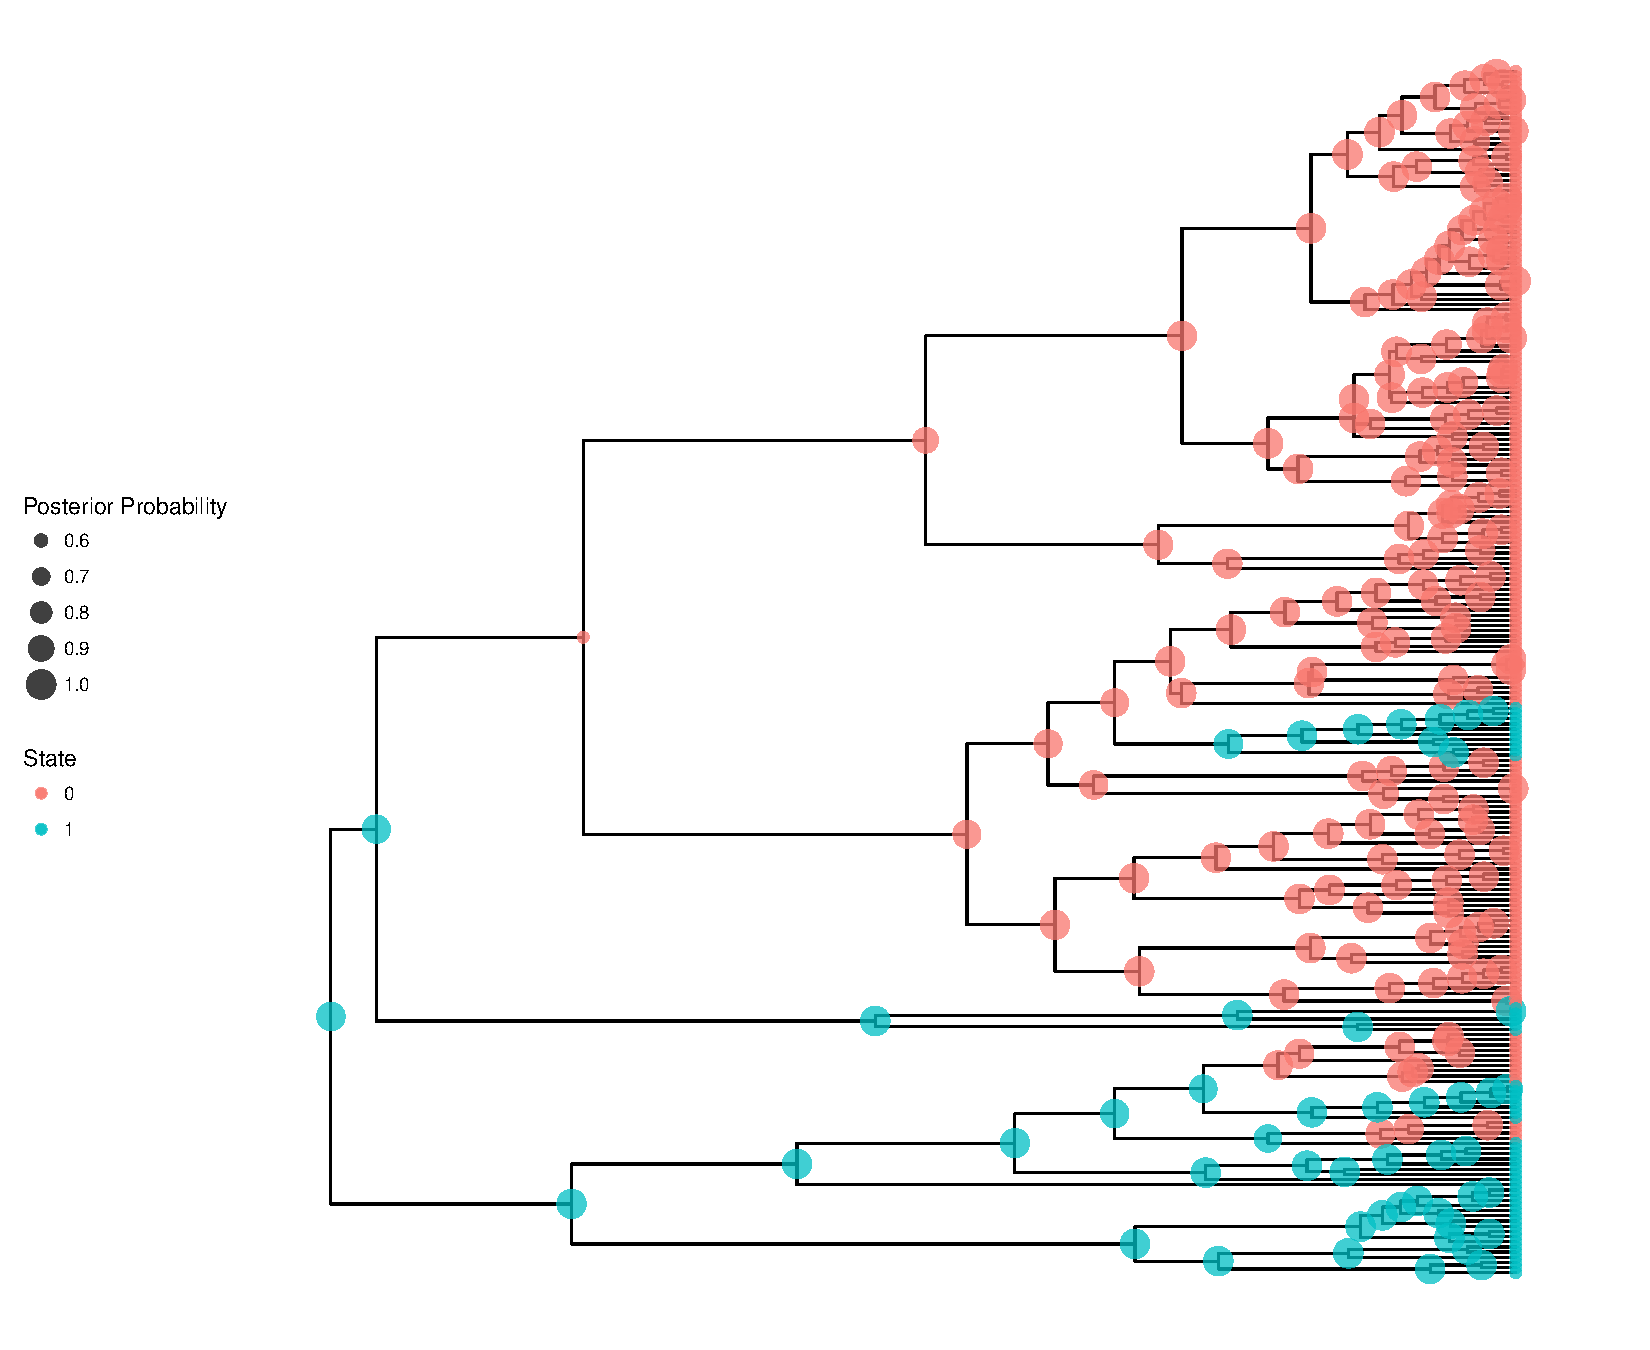
\includegraphics[width=\textwidth]{\ResourcePath figures/RevBayes_Anc_States_BiSSE.pdf}}
\caption{\small Estimated ancestral states for the activity period of primates.}
\label{fig:anc_states_BiSSE}
\end{figure}
The resulting plot is shown in Figure~\ref{fig:anc_states_BiSSE}.
We see both the maximum \emph{a posteriori} (MAP) estimate for each node as well as the posterior probability of the states represented by the size of the dots.


\subsubsection{Plotting diversification rates}
Now let us plot the diversification rate estimates.
Again, we are going to use \R for our plotting.
Specifically, we will use the package \texttt{ggplot2} but you can also use any other package that you prefer.
We are only taking advantage of reading in the tab-delimited file as a table and plot the different diversification rate parameters.
Note that we also rely on another provided \R script for plotting multiply plots in one file.
\definecolor{shadecolor}{RGB}{200,200,200}
{\tt \begin{snugshade*}
\begin{lstlisting}
library(ggplot2)
source("scripts/multiplot.R")

data <- read.table("output/primates_BiSSE.log",header=TRUE)

dat_ext  <- data.frame(dens = c(data$extinction.1, data$extinction.2), Type = rep(c("1", "2"), each = length(data$extinction.1)))
dat_spec <- data.frame(dens = c(data$speciation.1, data$speciation.2), Type = rep(c("1", "2"), each = length(data$extinction.1)))
dat_div  <- data.frame(dens = c(data$speciation.1-data$extinction.1, data$speciation.2-data$extinction.2), Type = rep(c("1", "2"), each = length(data$extinction.1)))
dat_rel  <- data.frame(dens = c(data$extinction.1/data$speciation.1, data$extinction.2/data$speciation.2), Type = rep(c("1", "2"), each = length(data$extinction.1)))

pdf("RevBayes_BiSSE_Results.pdf")

p1 <- ggplot(dat_spec, aes(x = dens, fill = Type)) + labs(title = "Speciation", x="Rate", y="Posterior Density") + geom_density(alpha = 0.5)
p2 <- ggplot(dat_ext, aes(x = dens, fill = Type)) + labs(title = "Extinction", x="Rate", y="Posterior Density") + geom_density(alpha = 0.5)
p3 <- ggplot(dat_div, aes(x = dens, fill = Type)) + labs(title = "Net-Diversification", x="Rate", y="Posterior Density") + geom_density(alpha = 0.5)
p4 <- ggplot(dat_rel, aes(x = dens, fill = Type)) + labs(title = "Relative Extinction", x="Rate", y="Posterior Density") + geom_density(alpha = 0.5)

multiplot(p1, p2, p3, p4)
dev.off()
\end{lstlisting}
\end{snugshade*}}
\begin{figure}[h!]
\centering
\fbox{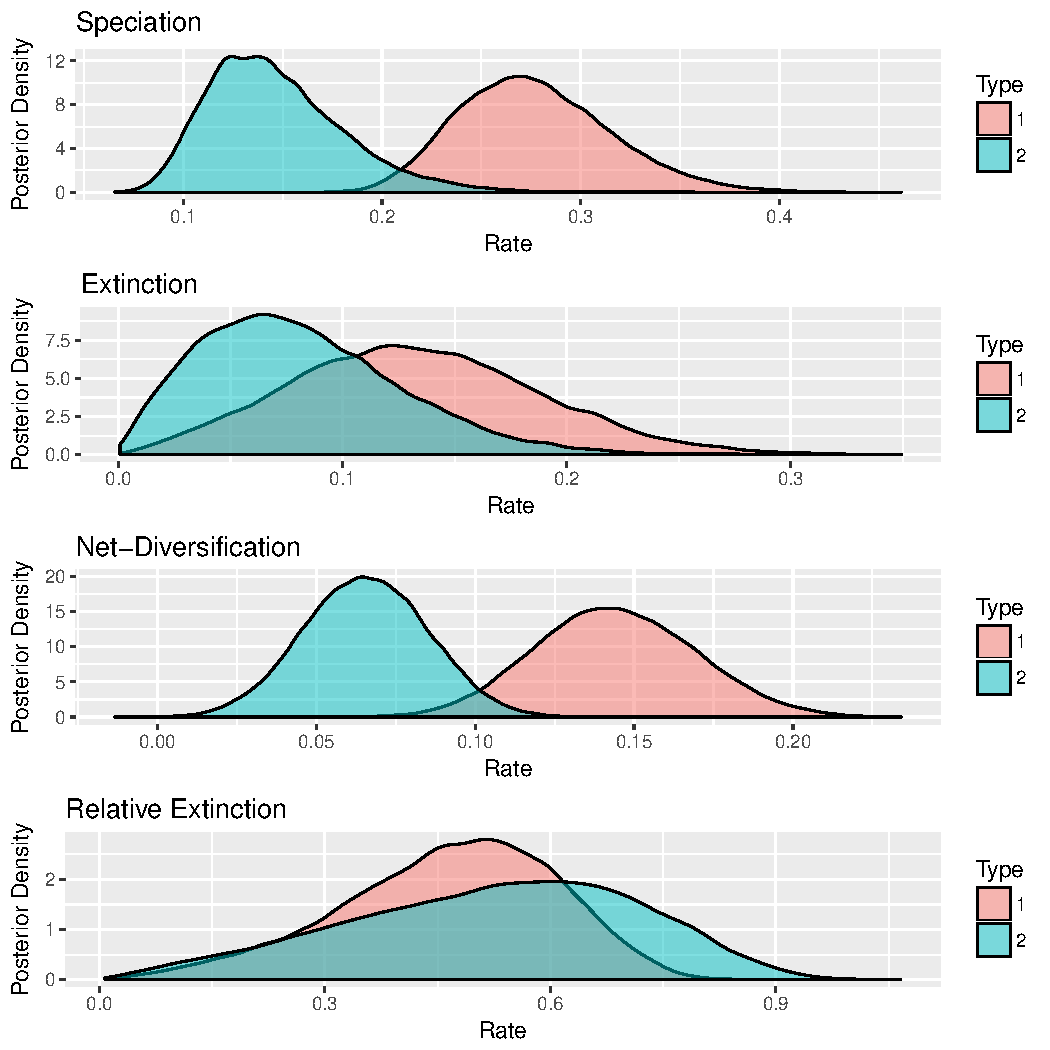
\includegraphics[width=\textwidth]{\ResourcePath figures/RevBayes_BiSSE_Results_activity_period.pdf}}
\caption{\small Estimated diversification rate for activity period (state 1 = Diurnal and state 2 = Nocturnal). We see that there is a nice difference in the estimated speciation rates but only little difference in the estimated}
\label{fig:anc_states_BiSSE}
\end{figure}


\definecolor{shadecolor}{RGB}{183,207,237}

%\impmark{The \Rev file for performing this analysis: \href{https://github.com/revbayes/revbayes_tutorial/raw/master/RB_DiversificationRateEpisodic_Tutorial/RevBayes_scripts/mcmc_EBD.Rev}{\cl{mcmc\_EBD.Rev}}.}
%\impmark{An \R file for plotting the output: \href{https://github.com/revbayes/revbayes_tutorial/raw/master/RB_DiversificationRateEpisodic_Tutorial/RevBayes_scripts/Plot_EBD_RevBayes.R}{\cl{Plot\_EBD\_RevBayes.R}}.}


\subsection{Exercise}

\begin{enumerate}
\item Run an MCMC simulation to estimate the posterior distribution of the speciation rate and extinction rate.
\item Visualize the state-specific diversification rates using \R.
\item Do you see evidence for rate differences between the two states?
\item Repeat this analysis for a different binary morphological character.
\end{enumerate}


\bigskip
\section{Accommodating uncorrelated diversification rate changes}\label{sec:HiSSE_Theory}

\RevBayes implements the multi-state extension of \BiSSE, just as implemented in \diversitree. 
The main differences are just which priors you use on the parameters and the inference procedure, \IE the specifics of the MCMC algorithm.
Here we will first describe the general theory about the model, borrowing heavily from the supplementary material of \cite{Moore2016}.
You may want to skip over this section if you are not interested in math behind.
Then we will show how to run this analysis in \RevBayes.
\begin{figure}[h!]
\centering
\fbox{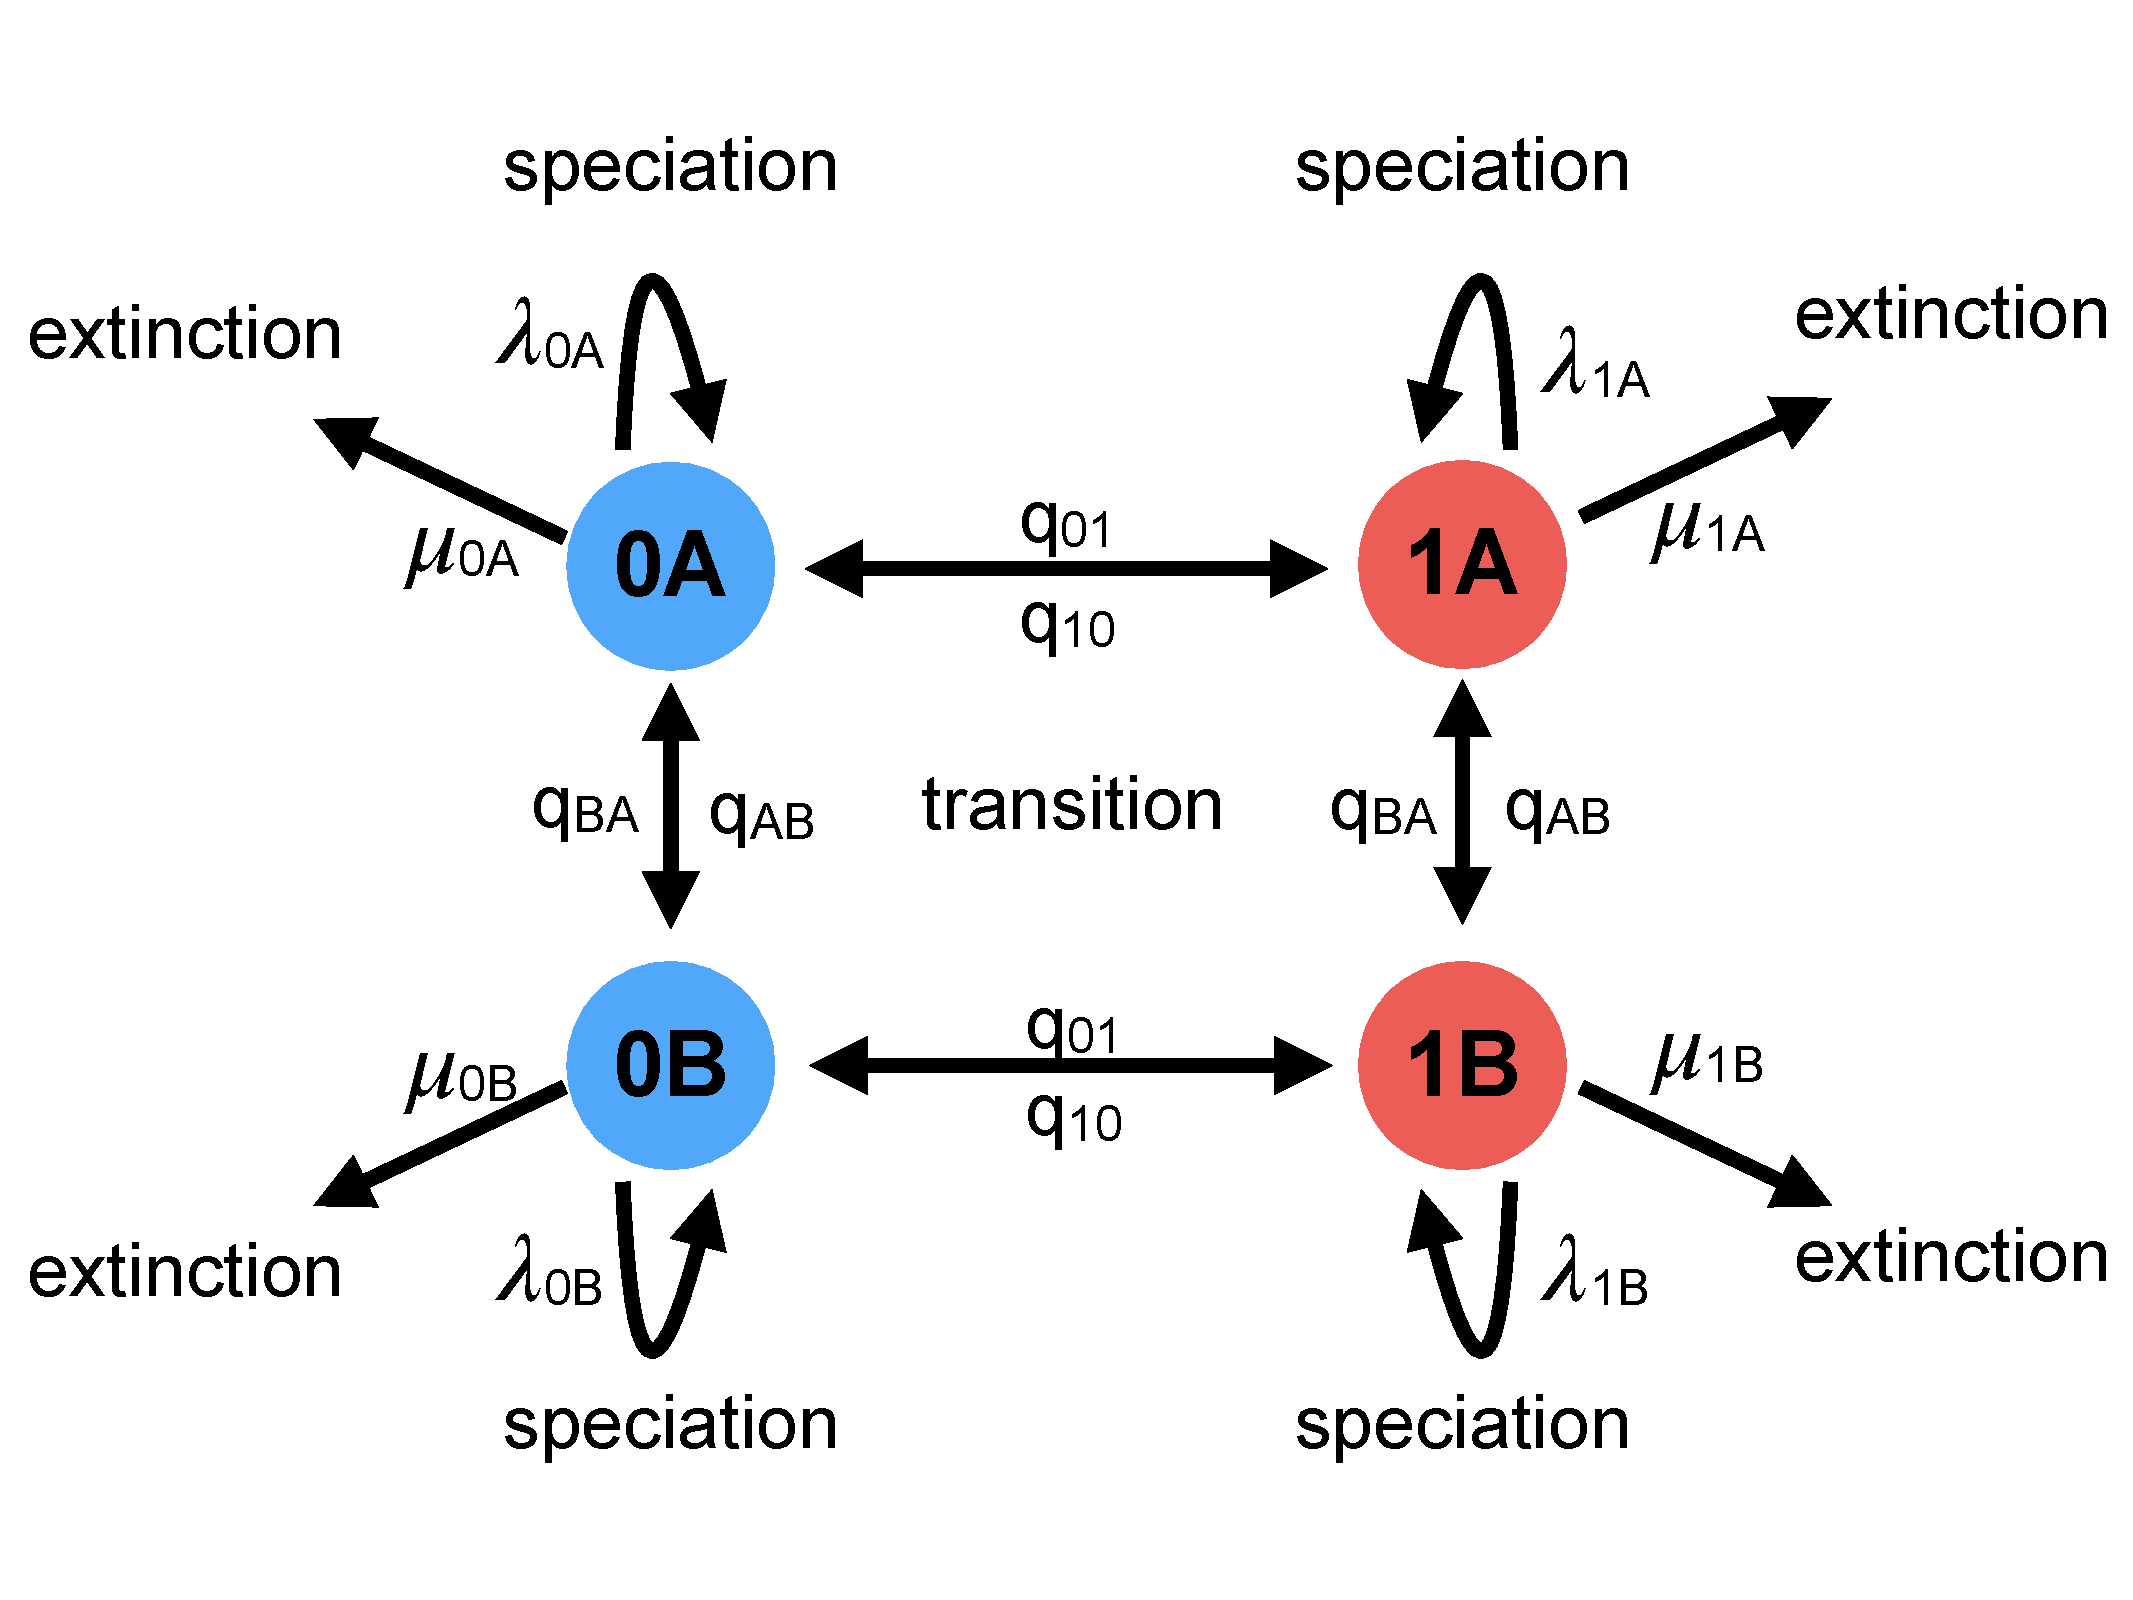
\includegraphics[width=\textwidth]{\ResourcePath figures/HiSSE.pdf}}
\caption{\small A schematic overview of the \HiSSE model. Each lineage has a binary state associated to it and thus can either be in state 0 (blue) or state 1 (red). When a lineage is in state 0 (blue), it can either (a) speciate with rate $\lambda_0$ which results into two descendant lineage both being in state 0 (blue); (b) it can go extinct with rate $\mu_0$; or (c) it can switch the state to 1 (red) with rate $q_{01}$. The same type of events are possible when a lineage is in state 1 (red) but with rate $\lambda_1$, $\mu_1$, and $q_{10}$ respectively.}
\label{fig:HiSSE_Schematic}
\end{figure}



\begin{table}[t!]
	\centering
	\caption{\bf{\HiSSE model parameters and their interpretation}} \label{tab:param}
	\begin{tabular}{ l l l }
		\toprule
		Parameter & Interpretation \\
		\midrule
		$\Psi$ & Phylogenetic tree with divergence times.\\
		\rowcolor{gray!15} $T$ & The root age.\\
%		\rowcolor{gray!15} $\gamma$ & Prior mean of the Poisson rate $\Lambda$.\\
%		$\Lambda$ & Prior mean of the Poisson-distributed number $k$ of shift events.\\
		$q_{01}$ & The rate of shifts from 0 to 1.\\
		\rowcolor{gray!15} $q_{10}$ & The rate of shifts from 1 to 0.\\
		$\lambda_0$ & Speciation rate for state 0.\\
		\rowcolor{gray!15} $\mu_0$ & Extinction rate for state 0.\\
		$\lambda_1$ & Speciation rate for state 1.\\
		\rowcolor{gray!15} $\mu_1$ & Extinction rate for state 1.\\
	\end{tabular}
\end{table}


\subsection{Read the tree}

Begin by reading in the observed tree and the morphological data. 
We have both stored in separate nexus files.
{\tt \begin{snugshade*}
\begin{lstlisting}
observed_phylogeny <- readTrees("data/primates_tree.nex")[1]
data <- readCharacterData("data/primates_solitariness.nex")
\end{lstlisting}
\end{snugshade*}}
Note, the character-dependent birth-death process currently uses always the first character/site in the alignment file.
We have therefore split the morphological dataset into several small files that include only one morphological character each.

From the tree, we can get some helpful variables:
{\tt \begin{snugshade*}
\begin{lstlisting}
taxa <- observed_phylogeny.taxa()
\end{lstlisting}
\end{snugshade*}}

Additionally, we can initialize an iterator variable for our vector of moves and monitors:
{\tt \begin{snugshade*}
\begin{lstlisting}
mvi = 0
mni = 0
\end{lstlisting}
\end{snugshade*}}

Finally, we create a helper variable that specifies the number of states that the morphological character has.
{\tt \begin{snugshade*}
\begin{lstlisting}
NUM_STATES = 2
NUM_HIDDEN = 2
NUM_RATES = NUM_STATES * NUM_HIDDEN
\end{lstlisting}
\end{snugshade*}}
Using this variable we can easily change our script to use a different morphological character with a different number of states.
We will also use this variable in our second example on hidden-state speciation and extinction model. 


\subsubsection{Priors on rates}
We start by specifying prior distributions on the diversification rates.
We will assume here an identical prior distribution on the speciation and extinction rate.
Furthermore, we will use a normal distribution as the prior distribution on the log of the speciation and extinction rate.
Hence, we will use a mean of $\frac{\ln(\frac{\text{\#Taxa}}{2})}{\text{tree-age}}$ which is the expected net-diversification rate.
{\tt \begin{snugshade*}
\begin{lstlisting}
rate_mean <- ln( ln(367.0/2.0) / observed_phylogeny.rootAge() )
rate_sd <- 2.0
\end{lstlisting}
\end{snugshade*}}
Now we can specify our character-specific specification and extinction rate parameters.
As we just said before, we are going to use normal distributions for the prior on the log-speciation and log-extinction rate.
Here we will use a \cl{for}-loop to specify speciation and extinction parameters for each character, \EG two in a binary state case.
{\tt \begin{snugshade*}
\begin{lstlisting}
for (i in 1:NUM_STATES) {
    
     ### Create a lognormal distributed variable for the diversification rate
    log_speciation[i] ~ dnNormal(mean=rate_mean,sd=rate_sd) 
    speciation[i] := exp( log_speciation[i] )
    moves[++mvi] = mvSlide(log_speciation[i],delta=0.20,tune=true,weight=3.0)

    ### Create a lognormal distributed variable for the turnover rate
    log_extinction[i] ~ dnNormal(mean=rate_mean,sd=rate_sd) 
    extinction[i] := exp( log_extinction[i] )
    moves[++mvi] = mvSlide(log_extinction[i],delta=0.20,tune=true,weight=3.0)

}
\end{lstlisting}
\end{snugshade*}}
Now we need to create the variable for the hidden states.
{\tt \begin{snugshade*}
\begin{lstlisting}
for (i in 1:(NUM_HIDDEN-1)) {
    
    ### Create an exponential distributed variable for the diversification rate
    speciation_beta[i] ~ dnExp(1.0) 
    moves[++mvi] = mvScale(speciation_beta[i],lambda=0.20,tune=true,weight=2.0)        

    ### Create an normal distributed variable for the turnover rate
    extinction_beta[i] ~ dnNormal(0.0,1.0)
    moves[++mvi] = mvSlide(extinction_beta[i],delta=0.20,tune=true,weight=2.0)
    
}
\end{lstlisting}
\end{snugshade*}}
Finally, we match the rates to all possible ---hidden and observed--- states.
{\tt \begin{snugshade*}
\begin{lstlisting}
for (j in 1:NUM_HIDDEN) {
    for (i in 1:NUM_STATES) {
        if ( j == 1) {
            speciation[i] := exp( speciation_alpha[i] )
            extinction[i] := exp( extinction_alpha[i] )
        } else {
            index = i+(j*NUM_STATES)-NUM_STATES
            speciation[index] := speciation[index-NUM_STATES] * exp( speciation_beta[j-1] )
            extinction[index] := exp( extinction_alpha[i] + extinction_beta[j-1] )
        }
    }
}
\end{lstlisting}
\end{snugshade*}}
As before, we specify a rate prior.
{\tt \begin{snugshade*}
\begin{lstlisting}
rate_pr := observed_phylogeny.treeLength() / 10
rate_12 ~ dnExponential(rate_pr)
rate_21 ~ dnExponential(rate_pr)
\end{lstlisting}
\end{snugshade*}}
For both rate variable we specify a scaling move.
{\tt \begin{snugshade*}
\begin{lstlisting}
moves[++mvi] = mvScale( rate_12, weight=2 )
moves[++mvi] = mvScale( rate_21, weight=2 )
\end{lstlisting}
\end{snugshade*}}
Finally, we build a rate matrix for the relative-rate of change between categories.
This is because we need a rate matrix in our state-dependent birth-death process.
{\tt \begin{snugshade*}
\begin{lstlisting}
Q := [ rate_12, rate_21 ]
\end{lstlisting}
\end{snugshade*}}
Set up the transition rate matrix for hidden states.
We assume the transitions among the hidden states are all equal and drawn from an exponential distribution.
{\tt \begin{snugshade*}
\begin{lstlisting}
hidden_rate ~ dnExponential(rate_pr)
moves[++mvi] = mvScale(hidden_rate,lambda=0.2,tune=true,weight=5)

for (i in 1:(NUM_HIDDEN * (NUM_HIDDEN - 1))) {
    R[i] := hidden_rate
}
\end{lstlisting}
\end{snugshade*}}
Create the rate matrix for the combined observed and hidden states
{\tt \begin{snugshade*}
\begin{lstlisting}
rate_matrix := fnHiddenStateRateMatrix(Q, R, rescaled=false)
\end{lstlisting}
\end{snugshade*}}
A specific note here is that we do not rescale the rate matrix. 
This is very important because otherwise rate matrices, as used for molecular evolution, are always rescaled to have an average rate of 1.0.
If such a rescaled rate matrix was used, then you need to provide an overall rate scalar $\delta$.

\subsubsection{Prior on the root state}
Create a variable with the prior probabilities of each rate category at the root.
We are using a flat Dirichlet distribution as the prior on each state.
In this case we are actually estimating the prior frequencies of the root states.
There has been some discussion about this in \cite{FitzJohn2009}.
You could also fix the prior probabilities for the root states to be equal (generally not recommended), or use empirical state frequencies. 
{\tt \begin{snugshade*}
\begin{lstlisting}
rate_category_prior ~ dnDirichlet( rep(1,NUM_STATES) )
moves[++mvi] = mvDirichletSimplex(rate_category_prior,tune=true,weight=2)
\end{lstlisting}
\end{snugshade*}}

\subsubsection{Incomplete Taxon Sampling}

We know that we have sampled 233 out of 367 living primate species. 
To account for this we can set the sampling parameter as a constant node with a value of 233/367
{\tt \begin{snugshade*}
\begin{lstlisting}
rho <- observed_phylogeny.ntips()/367
\end{lstlisting}
\end{snugshade*}}


\subsubsection{Root age}

The birth-death process requires a parameter for the root age.
In this exercise we use a fix tree and thus we know the age of the tree.
Hence, we can get the value for the root from the \citet{MagnusonFord2012} tree.
{\tt \begin{snugshade*}
\begin{lstlisting}
root <- observed_phylogeny.rootAge()
\end{lstlisting}
\end{snugshade*}}

\subsubsection{The time tree}

Now we have all of the parameters we need to specify the full episodic birth-death model. 
We initialize the stochastic node representing the time tree.
{\tt \begin{snugshade*}
\begin{lstlisting}
timetree ~ dnCDBDP( rootAge           = root,
                    speciationRates   = speciation,
                    extinctionRates   = extinction, 
                    Q                 = rate_matrix,
                    pi                = rate_category_prior,
                    delta             = 1.0,
                    rho               = rho,
                    condition         = "survival",
                    taxa              = taxa )
\end{lstlisting}
\end{snugshade*}}
And then we attach data to it.
{\tt \begin{snugshade*}
\begin{lstlisting}
timetree.clamp( observed_phylogeny )
timetree.clampCharData( data )
\end{lstlisting}
\end{snugshade*}}

Finally, we create a workspace object of our whole model using the \cl{model()} function. 
{\tt \begin{snugshade*}
\begin{lstlisting}
mymodel = model(rate_matrix)
\end{lstlisting}
\end{snugshade*}}

The \cl{model()} function traversed all of the connections and found all of the nodes we specified. 


\subsection{Running an MCMC analysis}

\subsubsection{Specifying Monitors}

For our MCMC analysis, we set up a vector of \emph{monitors} to record the states of our Markov chain. 
For more details 
{\tt \begin{snugshade*}
\begin{lstlisting}
monitors[++mni] = mnModel(filename="output/primates_HiSSE.log", printgen=1)
monitors[++mni] = mnJointConditionalAncestralState(tree=timetree, cdbdp=timetree, type="NaturalNumbers", printgen=1, withTips=true, withStartStates=false, filename="output/anc_states_primates_HiSSE.log")
monitors[++mni] = mnScreen(printgen=100, Q, R)
\end{lstlisting}
\end{snugshade*}}

\subsubsection{Initializing and Running the MCMC Simulation}

With a fully specified model, a set of monitors, and a set of moves, we can now set up the MCMC algorithm that will sample parameter values in proportion to their posterior probability. 
The \cl{mcmc()} function will create our MCMC object:
{\tt \begin{snugshade*}
\begin{lstlisting}
mymcmc = mcmc(mymodel, monitors, moves)
\end{lstlisting}
\end{snugshade*}}

First, we will run a pre-burnin to tune the moves and to obtain starting values from the posterior distribution.
{\tt \begin{snugshade*}
\begin{lstlisting}
mymcmc.burnin(generations=5000,tuningInterval=200)
\end{lstlisting}
\end{snugshade*}}

Now, run the MCMC:
{\tt \begin{snugshade*}
\begin{lstlisting}
mymcmc.run(generations=20000)
\end{lstlisting}
\end{snugshade*}}


\subsubsection{Summarizing ancestral states}
After the MCMC run we summarize and estimate the joint-ancestral-state estimates.
{\tt \begin{snugshade*}
\begin{lstlisting}
anc_states = readAncestralStateTrace("output/anc_states_primates_HiSSE.log")
anc_tree = ancestralStateTree(tree=observed_phylogeny, ancestral_state_trace_vector=anc_states, include_start_states=false, file="output/anc_states_primates_HiSSE_results.tree", burnin=0, summary_statistic="MAP", site=0)
\end{lstlisting}
\end{snugshade*}}



\subsubsection{Plotting diversification rates}
Again, we plot the diversification rate as before.
\definecolor{shadecolor}{RGB}{200,200,200}
{\tt \begin{snugshade*}
\begin{lstlisting}
library(ggplot2)
source("scripts/multiplot.R")

data <- read.table("output/primates_HiSSE.log",header=TRUE)

start <- round(0.5*length(data$extinction.1))
end   <- length(data$extinction.1)

HiSSE_types <- rep(c("1A", "2A", "1B", "2B"), each = length(data$extinction.1[start:end]))
dat_ext  <- data.frame(dens = c(data$extinction.1[start:end], data$extinction.2[start:end], data$extinction.3[start:end], data$extinction.4[start:end]), Type = HiSSE_types)
dat_spec <- data.frame(dens = c(data$speciation.1[start:end], data$speciation.2[start:end], data$speciation.3[start:end], data$speciation.4[start:end]), Type = HiSSE_types)
dat_div  <- data.frame(dens = c(data$speciation.1[start:end]-data$extinction.1[start:end], data$speciation.2[start:end]-data$extinction.2[start:end], data$speciation.3[start:end]-data$extinction.3[start:end], data$speciation.4[start:end]-data$extinction.4[start:end]), Type = HiSSE_types)
dat_rel  <- data.frame(dens = c(data$extinction.1[start:end]/data$speciation.1[start:end], data$extinction.2[start:end]/data$speciation.2[start:end], data$extinction.3[start:end]/data$speciation.3[start:end], data$extinction.4[start:end]/data$speciation.4[start:end]), Type = HiSSE_types)


pdf("RevBayes_HiSSE_Results.pdf")

p1 <- ggplot(dat_spec, aes(x = dens, fill = Type)) + labs(title = "Speciation", x="Rate", y="Posterior Density") + geom_density(alpha = 0.5) + guides(fill=guide_legend(ncol=2,byrow=TRUE))
p2 <- ggplot(dat_ext, aes(x = dens, fill = Type)) + labs(title = "Extinction", x="Rate", y="Posterior Density") + geom_density(alpha = 0.5) + guides(fill=guide_legend(ncol=2,byrow=TRUE))
p3 <- ggplot(dat_div, aes(x = dens, fill = Type)) + labs(title = "Net-Diversification", x="Rate", y="Posterior Density") + geom_density(alpha = 0.5) + guides(fill=guide_legend(ncol=2,byrow=TRUE))
p4 <- ggplot(dat_rel, aes(x = dens, fill = Type)) + labs(title = "Relative Extinction", x="Rate", y="Posterior Density") + geom_density(alpha = 0.5) + guides(fill=guide_legend(ncol=2,byrow=TRUE))

multiplot(p1, p2, p3, p4)
dev.off()


\end{lstlisting}
\end{snugshade*}}
\begin{figure}[h!]
\centering
\fbox{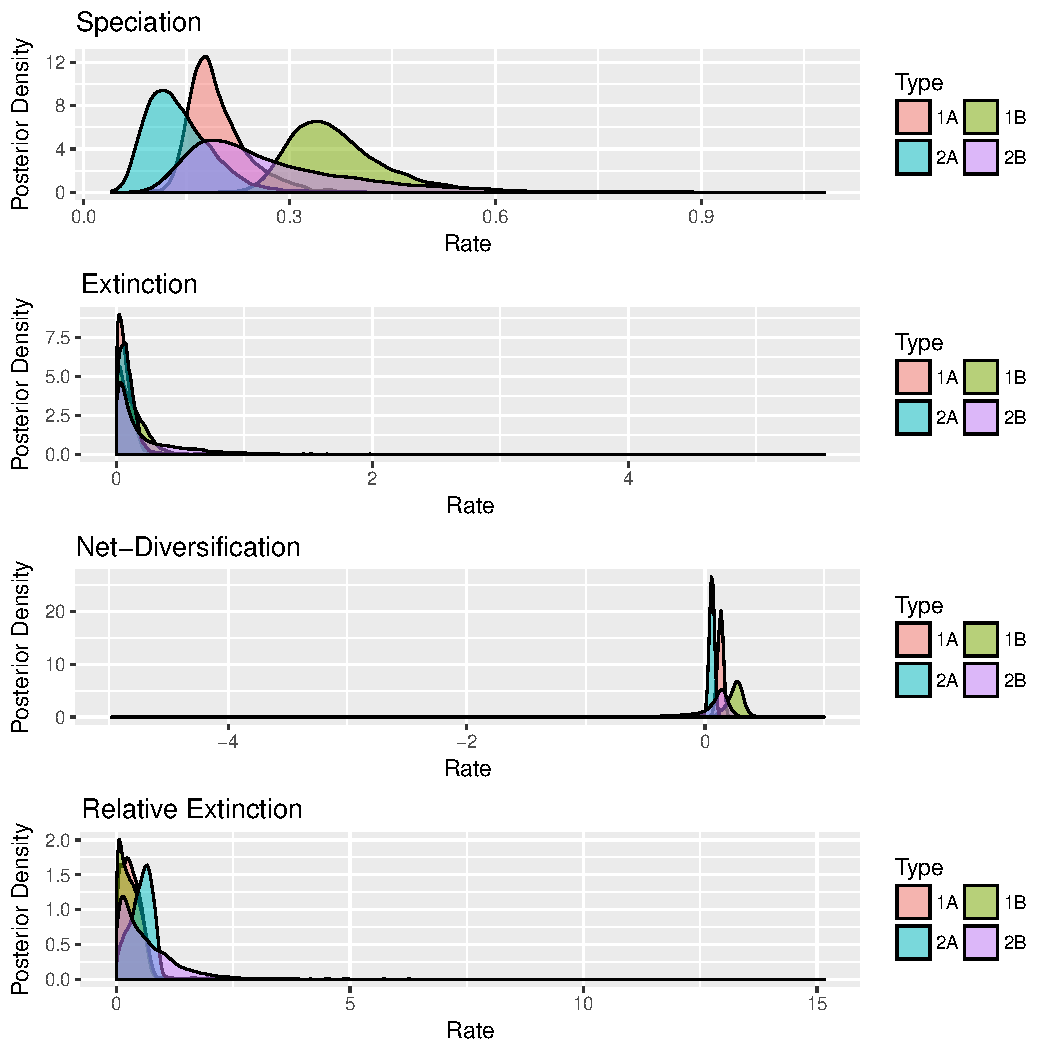
\includegraphics[width=\textwidth]{\ResourcePath figures/RevBayes_HiSSE_Results.pdf}}
\caption{\small Estimated diversification rate for activity period (state 1 = Diurnal and state 2 = Nocturnal). We see that there is a nice difference in the estimated speciation rates but only little difference in the estimated}
\label{fig:anc_states_BiSSE}
\end{figure}


\definecolor{shadecolor}{RGB}{183,207,237}

%\impmark{The \Rev file for performing this analysis: \href{https://github.com/revbayes/revbayes_tutorial/raw/master/RB_DiversificationRateEpisodic_Tutorial/RevBayes_scripts/mcmc_EBD.Rev}{\cl{mcmc\_EBD.Rev}}.}
%\impmark{An \R file for plotting the output: \href{https://github.com/revbayes/revbayes_tutorial/raw/master/RB_DiversificationRateEpisodic_Tutorial/RevBayes_scripts/Plot_EBD_RevBayes.R}{\cl{Plot\_EBD\_RevBayes.R}}.}


\subsection{Exercise}

\begin{enumerate}
\item Run an MCMC simulation to estimate the posterior distribution of the speciation rate and extinction rate.
\item Visualize the state-specific diversification rates using \R.
\item Do you see evidence for rate differences between the two states?
\item Do you see differences to the previous \BiSSE estimates?
\item Repeat this analysis for a different binary morphological character.
\end{enumerate}


\bigskip

\bibliographystyle{sysbio}
\bibliography{\GlobalResourcePath refs}
